\documentclass{article}

\usepackage[eandd]{neurips_2026}

\usepackage[utf8]{inputenc}
\usepackage[T1]{fontenc}
\usepackage{hyperref}
\usepackage{url}
\usepackage{booktabs}
\usepackage{amsmath}
\usepackage{amsfonts}
\usepackage{microtype}
\usepackage{xcolor}
\usepackage{graphicx}
\usepackage{tabularx}
\usepackage{makecell}
\usepackage{array}
\usepackage{tikz}
\usepackage{float}
\hypersetup{hidelinks}
\usetikzlibrary{arrows.meta,positioning,shapes.misc}

\title{Auditing Quality-Conditioned Structural-Prior Claims in Code Generation}

\author{Anonymous Authors}

\newcolumntype{Y}{>{\raggedright\arraybackslash}X}
\newcommand{\mbpp}{\textsc{MBPP}}
\newcommand{\code}[1]{\texttt{#1}}

\begin{document}
\maketitle

\begin{abstract}
Structural priors can guide few-shot code generation, but their evaluation is confounded when structural prompting, information access, candidate budget, prior quality, and execution-based selection change together. We study this as an evaluation-design problem: after controlling test-time opportunity and disclosing information access, which structural-prior claim remains warranted? We introduce SPC-Audit, a matched-budget diagnostic audit protocol for structural-prior claims in execution-evaluated Python function generation. The protocol matches candidate budget and execution-call accounting, reports prompt-token differences rather than claiming full compute equality, separates diagnostic from deployable selection, includes prompt-only and bad-prior boundary controls, and records explicit non-claims. On MBPP+224, an uncontrolled comparison suggests a large gain, $167/224 \rightarrow 184/224$; under the controlled diagnostic comparison, the supported positive claim narrows to fixed code-aware \code{syntax\_aware} episodes, where \code{no\_prior + MBR} solves $178.67 \pm 0.58$ tasks and \code{multi\_prior + MBR} solves $185.00 \pm 1.73$. The average gain is modest but directionally consistent across the three seeds, and paired query-seed outcomes are positive (30 improved, 11 regressed). The audit further identifies a quality-conditioned evaluation claim: under this protocol, intended code-aware priors show most positive movement in medium/high retrospective-fidelity bins, while more than half of \code{multi\_prior} cases remain low fidelity; the full prompt-only structural rerun is non-positive and rarely constructs high-fidelity priors; and misleading priors fall below the no-prior baseline. We therefore argue that structural-prior evaluations should report prior-quality coverage, quality-conditioned net delta, harm rate, claim survival, and explicit non-claims, not only average prior-versus-no-prior deltas. The contribution is a reusable E\&D reporting pattern and claim-audited artifact, not a deployable structural-prior method, new benchmark, strongest-method result, broad-transfer result, or backend-invariance claim.
\end{abstract}

\section{Introduction}
Execution-based benchmarks have made few-shot code generation increasingly measurable. Benchmarks such as MBPP, HumanEval, EvalPlus, and BigCodeBench evaluate generated programs by running tests rather than relying only on surface-form similarity \citep{austin2021program,chen2021evaluating,liu2023evalplus,zhuo2024bigcodebench}. At the same time, structure-aware code-generation pipelines add signals such as syntax-aware retrieval, program-structure summaries, or structural hints \citep{zhang2023syntax,tipirneni2022structcoder}. These signals are natural for code, but they are often evaluated in pipelines that also change retrieval information access, candidate budget, prior construction, and test-time execution selection.

The difficulty is attribution. A higher solved-task count does not by itself show whether the improvement should be attributed to structural conditioning, extra candidate-generation opportunity, code-aware retrieval, same-test execution selection, or the quality of the supplied prior. This problem is especially acute for structural priors because a prior is not merely present or absent: it may be high fidelity, low fidelity, or actively misleading.

We therefore treat evaluation design as the object of study. We ask which structural-prior claim survives after candidate budget, execution-call accounting, information access, selection status, prompt-only controls, bad-prior controls, and diagnostic prior quality are made explicit. We call the resulting reporting pattern SPC-Audit: Structural-Prior Claim Audit. SPC-Audit is not a new benchmark, generation model, deployable retrieval method, or strongest-method claim. It is a diagnostic protocol for auditing which claims remain warranted under specified assumptions about budget, information access, selection, and prior quality.

The central empirical lesson is a quality-conditioned evaluation claim. In the main controlled comparison, intended code-aware priors yield a modest positive diagnostic effect. However, prompt-only structural retrieval does not reproduce the effect on full MBPP+224, and misleading priors fall below the no-prior baseline. A retrospective prior-quality response audit reconciles these observations: for intended code-aware priors, most positive movement appears in medium/high diagnostic-fidelity bins, whereas the full prompt-only rerun rarely constructs high-fidelity priors. This should be interpreted as an E\&D claim about what the evaluation must measure, not as a causal mechanism proof or a deployable prior-quality estimator.

This framing yields three contributions. First, we provide SPC-Audit, a matched-budget diagnostic audit protocol for structural-prior claims with explicit information-access and selector-status disclosure. Second, we show a conclusion shift on MBPP+224: a large uncontrolled gain narrows to a modest fixed code-aware diagnostic effect, while full prompt-only structural retrieval remains unsupported. Third, we provide a quality-response reporting artifact: structural-prior evaluations should report prior-quality coverage, quality-conditioned net delta, harm rate, threshold sensitivity, paired directionality, survived claims, and explicit non-claims rather than only an average prior-versus-no-prior delta.

\begin{figure}[H]
\centering
\resizebox{\linewidth}{!}{%
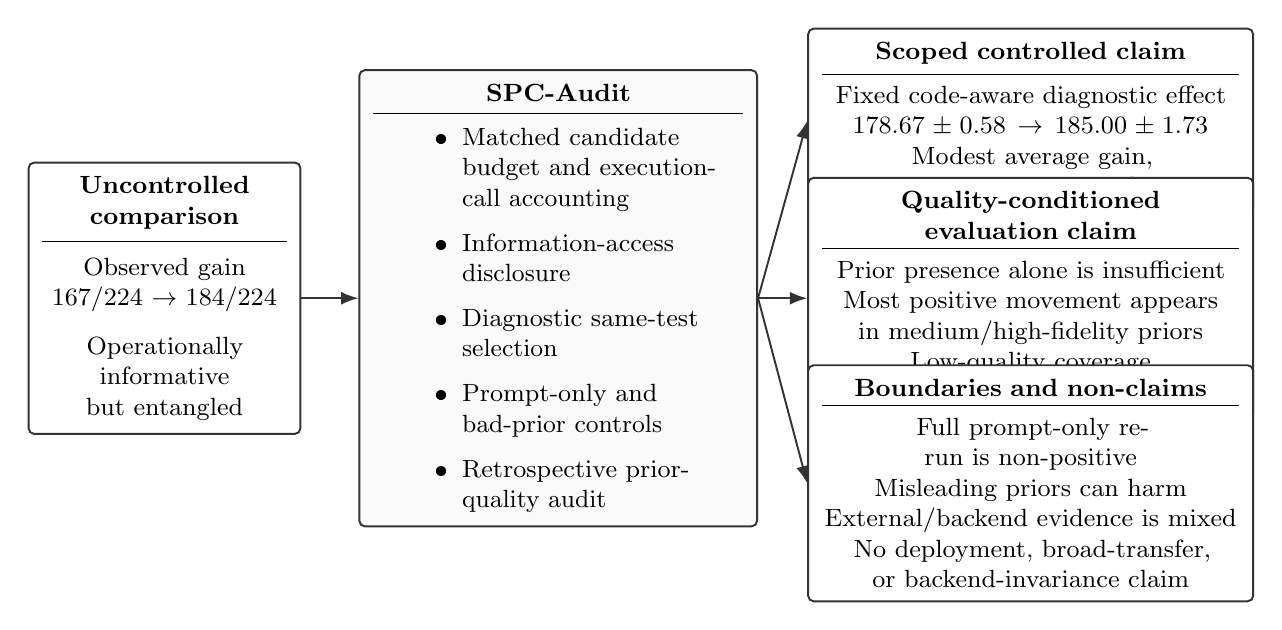
\begin{tikzpicture}[
  font=\small,
  box/.style={draw=black!80, rounded corners=2pt, line width=0.7pt, align=center, fill=white, inner sep=5pt},
  header/.style={font=\bfseries\small},
  arr/.style={-{Latex[length=2.2mm]}, line width=0.7pt, draw=black!80},
  bullet/.style={align=left, text width=4.0cm}
]
\node[box, text width=3.1cm, minimum height=2.9cm] (un) at (0,0) {\textbf{Uncontrolled comparison}\\[0.45em]\hrule\vspace{0.65em}Observed gain\\$167/224 \rightarrow 184/224$\\[0.7em]Operationally informative\\but entangled};
\node[box, text width=4.7cm, minimum height=4.4cm, fill=black!2] (audit) at (5.0,0) {\textbf{SPC-Audit}\\[0.45em]\hrule\vspace{0.55em}\begin{minipage}{4.2cm}\begin{itemize}\setlength\itemsep{0.35em}\setlength\leftmargini{1.1em}\item Matched candidate budget and execution-call accounting\item Information-access disclosure\item Diagnostic same-test selection\item Prompt-only and bad-prior controls\item Retrospective prior-quality audit\end{itemize}\end{minipage}};
\node[box, text width=5.3cm, minimum height=1.65cm] (c1) at (11.0,2.25) {\textbf{Scoped controlled claim}\\[0.35em]\hrule\vspace{0.45em}Fixed code-aware diagnostic effect\\$178.67 \pm 0.58 \rightarrow 185.00 \pm 1.73$\\Modest average gain, positive across seeds};
\node[box, text width=5.3cm, minimum height=1.75cm] (c2) at (11.0,0) {\textbf{Quality-conditioned evaluation claim}\\[0.35em]\hrule\vspace{0.45em}Prior presence alone is insufficient\\Most positive movement appears in medium/high-fidelity priors\\Low-quality coverage limits average gain};
\node[box, text width=5.3cm, minimum height=1.9cm] (c3) at (11.0,-2.35) {\textbf{Boundaries and non-claims}\\[0.35em]\hrule\vspace{0.45em}Full prompt-only rerun is non-positive\\Misleading priors can harm\\External/backend evidence is mixed\\No deployment, broad-transfer, or backend-invariance claim};
\draw[arr] (un.east) -- (audit.west);
\draw[arr] (audit.east) -- (c1.west);
\draw[arr] (audit.east) -- (c2.west);
\draw[arr] (audit.east) -- (c3.west);
\end{tikzpicture}%
}
\caption{Overview of the claim-audit logic. SPC-Audit turns an uncontrolled operational gain into a narrower supported claim, a quality-conditioned evaluation claim, and explicit boundaries/non-claims.}
\label{fig:claim-audit}
\end{figure}

\begin{table}[H]
\caption{Claim audit card and survival hierarchy. The paper supports a quality-conditioned evaluation claim rather than a deployable method or a broad structural-prior claim.}
\label{tab:claim-card}
\centering
\scriptsize
\begin{tabularx}{\linewidth}{l l Y Y}
\toprule
Claim & Status & Evidence in this paper & Boundary \\
\midrule
C0: operational pipeline gain & Supported but entangled & $167/224 \rightarrow 184/224$ & Operational comparison; not attributed. \\
C1: matched-budget code-aware diagnostic effect & Supported with scope & $178.67 \pm 0.58 \rightarrow 185.00 \pm 1.73$ & Fixed code-aware \code{syntax\_aware} episodes only. \\
C2: quality-conditioned evaluation claim & Diagnostic support & Intended priors are most positive in medium/high bins; prompt-only high-fidelity coverage is rare; bad priors regress. & Retrospective audit; not causal proof. \\
C3: full prompt-only structural retrieval & Not supported & $179.33 \pm 2.31$ vs. $177.67 \pm 1.53$ & Deployable prompt-only claim unsupported. \\
C4: broad transfer / strongest-method / backend-invariance & Unsupported & External and backend rows are mixed or replicate-sensitive. & Explicit non-claims. \\
\bottomrule
\end{tabularx}
\end{table}

\section{Related Work}
Execution-based code-generation benchmarks motivate our setting. MBPP and HumanEval established task-level program synthesis evaluation for generated Python functions \citep{austin2021program,chen2021evaluating}; EvalPlus strengthens evaluation by expanding test suites \citep{liu2023evalplus}; BigCodeBench broadens code-generation evaluation toward more complex instructions and function calls \citep{zhuo2024bigcodebench}. These benchmarks make outcome measurement more reliable, but they do not by themselves determine whether an observed improvement is attributable to structural conditioning, retrieval information, candidate budget, prior quality, or test-time selection.

Structure-aware and retrieval-augmented code-generation work motivates the structural-prior hypothesis. Syntax-aware retrieval and structure-aware code models suggest that program structure can provide useful conditioning information \citep{zhang2023syntax,tipirneni2022structcoder}. Our focus is not to introduce a stronger structural prior. Instead, we audit what claim remains when the evaluation controls candidate-generation opportunity, reports information access, and includes prompt-only, bad-prior, and quality-response boundaries.

Execution-guided selection and MBR-style selection motivate our treatment of MBR-exec as a diagnostic selector rather than as part of the structural prior \citep{shi2022execution,vamvas2024linear}. Because our selector executes candidates against packaged task tests and uses those same tests for reporting, it is appropriate for diagnostic attribution but not for a deployment-time selection claim.

Evaluation reporting and artifact documentation are also central to our framing. Prior work has argued that test-set scores alone can be insufficient for drawing accurate conclusions and that benchmark comparisons should account for sources of variation \citep{dodge2019show,bouthillier2021accounting}. Reproducibility and documentation frameworks further motivate clear code/data availability, provenance, intended-use reporting, and limitation statements \citep{pineau2021improving,gebru2021datasheets,mitchell2019model,bender2018data}. SPC-Audit follows this reporting-oriented tradition, but specializes it to structural-prior claims through matched-budget accounting, information-access disclosure, prompt-only and bad-prior controls, prior-quality response, and explicit non-claims.

\section{SPC-Audit: Matched-Budget Diagnostic Evaluation}
We study execution-evaluated few-shot Python function generation. Each evaluation instance is an episode containing a query task, an entry point, executable tests, and a fixed set of retrieved support examples. A generator produces candidate programs, and a selector chooses one candidate. The episode is counted as solved if the selected candidate passes the associated tests.

The protocol varies the prior condition while matching candidate budget and execution-call accounting. In the main MBPP+224 comparison, every condition uses \code{syntax\_aware} retrieval, one support example, candidate budget 8, execution budget 8, diagnostic MBR-exec selection, and seeds 1, 2, and 3. We compare \code{no\_prior}, \code{single\_prior}, \code{multi\_prior}, \code{random\_prior}, and \code{corrupted\_prior}. Matched budget in this paper means matched candidate budget and execution-call accounting; it does not imply matched prompt tokens, latency, wall-clock time, or full compute equality.

The information-access disclosure is part of the protocol. The main \code{syntax\_aware} episode construction uses stored query code fields and is therefore code-aware diagnostic evidence. Prompt-only lexical retrieval uses only query prompt text. Prompt-only structural retrieval uses only query prompt text and entry point on the query side, while allowing support-side structure from training-pool examples. \code{corrupted\_prior} is oracle-derived before corruption and is a diagnostic stress test, not a deployable method.

MBR-exec is also diagnostic. It executes candidates against packaged task tests and uses those same tests for candidate selection and solved-count reporting. Under the main comparison, every prior condition uses the same candidate budget and execution-selection regime. This makes the comparison suitable for E\&D attribution auditing, not for claiming a deployment-time selection system.

\begin{table}[H]
\caption{SPC-Audit reporting checklist. The checklist is a reusable E\&D reporting pattern rather than a new benchmark or deployable method.}
\label{tab:audit-checklist}
\centering
\footnotesize
\begin{tabularx}{\linewidth}{l Y}
\toprule
Audit item & Required reporting in this paper \\
\midrule
Candidate budget & Total candidates and split across prior variants. \\
Execution-call accounting & Executions available to each condition. \\
Prompt-token accounting & Token totals are reported; they are not matched. \\
Information access & Query/support fields used by retrieval, prompting, selection, and evaluation. \\
Selection status & Deployable, diagnostic, same-test, public-test, or oracle-like. \\
Prompt-only boundary & A condition without query solution code. \\
Bad-prior control & Random, corrupted, or misleading priors under the same selector. \\
Quality response & Coverage, bin-level net delta, harm rate, separation, and threshold sensitivity. \\
Explicit non-claims & No strongest-method, broad-transfer, backend-invariance, full-compute, deployable, or safety claim. \\
\bottomrule
\end{tabularx}
\end{table}

\section{Prior-Quality Response as an Evaluation Object}
A prior-versus-no-prior average delta is incomplete because a prior condition can look weak either because structural information is unhelpful or because the condition rarely constructs high-quality priors. A prior-quality response audit asks what quality of prior was supplied, how often medium/high-fidelity priors were constructed, whether changed outcomes are positive or negative inside each fidelity band, and whether low-quality or misleading priors increase regressions.

For a prior condition, we report five quantities: quality coverage, bin-level net delta, harm rate, outcome-level fidelity separation, and threshold sensitivity. Quality coverage is the fraction of query-seed outcomes in low, medium, or high diagnostic-fidelity bins. Bin-level net delta is improved minus regressed outcomes within a bin. Harm rate is regressed divided by changed outcomes. Outcome-level fidelity separation compares the mean diagnostic fidelity of improved and regressed outcomes without binning. Threshold sensitivity repeats the audit at fixed cutoffs.

In this paper, fidelity is measured by \code{structure\_fidelity}, a stored diagnostic field comparing query reference-code structure with the prior summary through API-call, control-flow, and data-structure overlap. Because it uses reference code, it is retrospective and non-deployable. It is therefore a diagnostic stratifier, not a deployable quality estimator. For intended priors it helps stratify outcome movement; for corrupted priors it also shows why structural overlap alone is insufficient.

The prompt-only structural matcher is fixed and deterministic. Query-side matching uses only task prompt text and entry point. Support-side matching may use training-pool support prompt, entry point, and support-code structure. The same formula and constants are used for both prompt-only structural controls, including the full MBPP+224 rerun. The reported full rerun is not selected from an alternative-weight sweep, and no alternative-weight sweep is used in the canonical artifact. It is a boundary control, not a new prior-construction method.

\section{Experimental Setup}
The main result uses Qwen/Qwen2.5-Coder-7B-Instruct through \code{vllm\_openai} on MBPP+224 \citep{hui2024qwen}. The main matched-budget table compares \code{no\_prior}, \code{single\_prior}, \code{multi\_prior}, \code{random\_prior}, and \code{corrupted\_prior} across seeds 1, 2, and 3. Candidate budget and execution budget are both 8; prompt-token totals are reported but not matched.

Supplementary boundary checks use MBPP+100, HumanEval+, BigCodeBench-Hard compatible slices, DeepSeek \citep{guo2024deepseek}, and StarCoder-family backends \citep{li2023starcoder}. These rows instantiate the reporting pattern and test sensitivity; they do not support backend invariance or broad transfer. We retain positive, neutral, mixed, and negative rows because the purpose is claim calibration rather than result selection.

\section{Results}
\subsection{Matched-budget evaluation narrows the claim}
The central result is a conclusion shift. Under the earlier uncontrolled comparison, the relevant contrast was $167/224 \rightarrow 184/224$, which is operationally informative but entangled because structural conditioning and execution-selection opportunity change together. Under matched candidate budget and execution-call accounting, the relevant contrast becomes $178.67 \pm 0.58 \rightarrow 185.00 \pm 1.73$. The average fair-budget gain is modest but consistently positive across the three seeds, and it should be interpreted as a scoped diagnostic effect in fixed code-aware episodes rather than as a broad structural-prior method claim.

Paired outcomes make the scope clearer. For \code{multi\_prior} versus \code{no\_prior}, the pooled query-seed comparison gives 30 improved, 11 regressed, and 631 unchanged outcomes, with positive net movement in all three seeds. Because query-seed outcomes are not fully independent, we also collapse by task: 14 tasks have positive net deltas, 5 have negative net deltas, and 205 are unchanged. We therefore interpret the result as positive but scoped directional evidence rather than as a robustness claim.

\begin{table}[H]
\caption{Main MBPP+224 matched-budget diagnostic comparison. All settings use candidate budget 8 and execution budget 8 with diagnostic MBR-exec. Prompt tokens are reported but not matched; this table does not claim full compute equality.}
\label{tab:main-result}
\centering
\footnotesize
\begin{tabular}{lrrrrrr}
\toprule
Setting & Solved mean & Range & $\Delta$ vs. no prior & Avg. cand. & Prompt tok. & Compl. tok. \\
\midrule
\code{no\_prior} & 178.67 & [178, 179] & +0.00 & 8.00 & 38261 & 14736 \\
\code{single\_prior} & 181.67 & [181, 183] & +3.00 & 8.00 & 46078 & 13182 \\
\code{multi\_prior} & 185.00 & [184, 187] & +6.33 & 8.00 & 46008 & 13195 \\
\code{random\_prior} & 172.33 & [172, 173] & -6.33 & 8.00 & 60193 & 13938 \\
\code{corrupted\_prior} & 173.33 & [172, 175] & -5.33 & 8.00 & 59927 & 13916 \\
\bottomrule
\end{tabular}
\end{table}

\subsection{A quality-conditioned evaluation claim}
The prior-quality response audit is the main reason to treat the prompt-only negative result as more than a defensive caveat. It shows that structural-prior effects are not well summarized by prior presence alone. For intended priors in fixed code-aware \code{syntax\_aware} episodes, most positive net movement appears in medium/high retrospective-fidelity bins. For \code{multi\_prior}, medium/high-fidelity cases cover 0.469 of query-seed outcomes, with 23 improvements, 6 regressions, net +17, and harm rate 0.207. In contrast, the low-fidelity bin has net +2. The modest average gain is therefore partly explained by limited prior-quality coverage: more than half of \code{multi\_prior} query-seed outcomes remain low fidelity, and most of the positive movement comes from the medium/high-fidelity subset. \code{single\_prior} shows the same directional pattern, though more weakly.

The bad-prior rows provide an important nuance. Random and corrupted priors are harmful even though structural overlap is not always minimal. This means \code{structure\_fidelity} is useful for intended-prior stratification, but it is not a complete quality metric. A prior can preserve some structural surface while still being misleading enough to increase regressions. We therefore frame the result as a quality-conditioned evaluation claim rather than a scalar-quality or causal-mechanism claim.

Threshold sensitivity supports the intended-prior interpretation without turning the thresholds into a tuning rule: for code-aware \code{multi\_prior}, thresholds 0.10, 0.15, 0.25, and 0.50 yield net deltas of +17, +17, +16, and +4. These checks remain retrospective and diagnostic.

\begin{table}[H]
\caption{Condensed prior-quality response card. Intended-prior rows support the quality-conditioned evaluation claim; bad-prior rows show that structural overlap alone is insufficient. The audit is retrospective and reference-code-based.}
\label{tab:quality-response}
\centering
\scriptsize
\begin{tabular}{llrrrrr}
\toprule
Regime / setting & Bin & Coverage & Improved & Regressed & Net & Harm \\
\midrule
Code-aware \code{single\_prior} & low & 0.603 & 9 & 10 & -1 & 0.526 \\
Code-aware \code{single\_prior} & med/high & 0.397 & 16 & 6 & +10 & 0.273 \\
Code-aware \code{multi\_prior} & low & 0.531 & 7 & 5 & +2 & 0.417 \\
Code-aware \code{multi\_prior} & med/high & 0.469 & 23 & 6 & +17 & 0.207 \\
Code-aware \code{random\_prior} & all & 1.000 & 25 & 44 & -19 & 0.638 \\
Code-aware \code{corrupted\_prior} & all & 1.000 & 34 & 50 & -16 & 0.595 \\
Prompt-only \code{single\_prior} & low & 0.808 & 12 & 23 & -11 & 0.657 \\
Prompt-only \code{single\_prior} & med/high & 0.192 & 4 & 10 & -6 & 0.714 \\
Prompt-only \code{multi\_prior} & low & 0.799 & 14 & 15 & -1 & 0.517 \\
Prompt-only \code{multi\_prior} & med/high & 0.201 & 4 & 8 & -4 & 0.667 \\
\bottomrule
\end{tabular}
\end{table}

\subsection{Prompt-only failure exposes a quality-coverage boundary}
Prompt-only controls bound the claim and make the quality-response view necessary. Lexical retrieval on MBPP+100 does not reproduce the effect: \code{no\_prior} and \code{single\_prior} both solve $81.50 \pm 0.71$, while \code{multi\_prior} solves $80.50 \pm 0.71$. A prompt-only structural control on MBPP+100 is weakly positive for \code{multi\_prior}: $82.50 \pm 2.12$ for \code{no\_prior}, $81.00 \pm 0.00$ for \code{single\_prior}, and $83.50 \pm 0.71$ for \code{multi\_prior}. The decisive full MBPP+224 prompt-only structural rerun is non-positive.

The full prompt-only \code{prompt\_structural} rerun has low diagnostic-fidelity coverage: only 6 of 672 \code{multi\_prior} query-seed outcomes reach the high-fidelity bin. This does not prove that low prior quality is the sole cause of the prompt-only failure. It does show that a structural-prior evaluation must report whether the protocol actually supplies high-fidelity priors often enough to support the claimed effect.

\begin{table}[H]
\caption{Prompt-only boundary controls. The full MBPP+224 prompt-only structural rerun is the claim-boundary row; it does not support deployable prompt-only structural retrieval.}
\label{tab:prompt-only}
\centering
\scriptsize
\begin{tabularx}{\linewidth}{l l l l l Y}
\toprule
Control & Dataset & no prior & single prior & multi prior & Interpretation \\
\midrule
Prompt-only lexical & MBPP+100 & $81.50 \pm 0.71$ & $81.50 \pm 0.71$ & $80.50 \pm 0.71$ & No positive prompt-only lexical effect. \\
Prompt-only structural & MBPP+100 & $82.50 \pm 2.12$ & $81.00 \pm 0.00$ & $83.50 \pm 0.71$ & Weak positive slice only. \\
Prompt-only structural & MBPP+224 & $179.33 \pm 2.31$ & $173.67 \pm 0.58$ & $177.67 \pm 1.53$ & Full rerun non-positive. \\
\bottomrule
\end{tabularx}
\end{table}

\subsection{Boundary checks prevent broader claims}
Stress and boundary analyses define the claim scope rather than robustness. The bad-prior controls provide the harm side of the quality-response claim: under the same candidate budget and diagnostic selector, \code{random\_prior} and \code{corrupted\_prior} solve $172.33 \pm 0.58$ and $173.33 \pm 1.53$ tasks, both below \code{no\_prior} at $178.67 \pm 0.58$. The multi-seed decomposition is provided in the artifact; regressions are dominated by all-candidate compile failure. We treat this as diagnostic proposal-quality evidence, not a deployment-safety or causal mechanism claim.

The MBPP+100 budget sweep shows varying ordering across budgets 1, 4, 8, and 16, so the main effect should not be interpreted as budget-invariant. HumanEval+164 supports non-degradation, not transfer. HumanEval+50 with DeepSeek is mixed across two seeds, giving a two-seed aggregate of $86/100$ versus $85/100$. BigCodeBench-Hard compatible slices are slice-sensitive: compatible30 is negative, $14/30$ versus $11/30$, while compatible50 is slightly positive, $22/50$ versus $23/50$. Cross-backend evidence is also boundary evidence. Qwen and DeepSeek provide same-scale MBPP+100 support, but StarCoder-family and local backend rows are replicate-sensitive or negative under weaker serving conditions.

\begin{table}[H]
\caption{Compact boundary instantiations. These checks define claim scope; they do not support broad transfer, backend invariance, budget invariance, deployment, or robustness.}
\label{tab:boundaries}
\centering
\footnotesize
\begin{tabularx}{\linewidth}{l Y Y}
\toprule
Boundary & Evidence & Interpretation \\
\midrule
Bad priors & \code{random\_prior} and \code{corrupted\_prior} are below \code{no\_prior} under the same diagnostic selector. & Misleading structure can harm; diagnostic proposal-quality evidence. \\
Budget & MBPP+100 sweep varies across budgets 1, 4, 8, 16. & Effects are budget-sensitive, not monotonic. \\
External slices & HumanEval+164 non-degradation; HumanEval+50 mixed; BigCodeBench-Hard slices mixed. & Compatibility/slice evidence, not broad transfer. \\
Backends & Qwen/DeepSeek support; local/weak backend rows mixed or negative. & Backend-aware audit evidence, not backend invariance. \\
\bottomrule
\end{tabularx}
\end{table}

\section{Artifact and Reproducibility}
The artifact is part of the E\&D contribution. It packages the claim-to-evidence map, raw-result provenance, table-regeneration scripts, matcher checks, prior-quality response tables, reusable audit templates, information-access cards, and known limitations. The reviewer quickstart runs \code{bash artifact/reproduce\_main.sh} to regenerate paper-facing tables and figure-support files from cached outputs, and \code{bash artifact/verify\_provenance.sh} to check prompt-only matcher constants, query-side access boundaries, stored \code{structure\_fidelity} fields, and prior-quality response regeneration. These scripts do not call an LLM and do not rebuild raw generations.

The artifact includes a verification log reporting PASS for cached table regeneration, matcher provenance checks, stored \code{structure\_fidelity} checks, and prior-quality audit regeneration. This supports artifact inspection and table provenance; it is not a claim that all raw LLM completions are regenerated without live inference.

The artifact distinguishes cached-output regeneration from live model reruns. The main benchmark and external evaluations are rerunnable under the matching live-inference assumption. Full live reruns require matching model endpoints or local models and should be run in an isolated environment because generated Python code is untrusted. Public data release follows a conservative policy: benchmark-derived resources are redistributed only when upstream permission is verified; otherwise the artifact provides preparation scripts, provenance notes, metadata, expected layout, and hashes.

\section{Limitations}
The scientific object is narrow: execution-evaluated few-shot Python function generation under fixed candidate budgets. The results do not cover repository-level generation, tool-use agents, multi-file synthesis, deployment safety, or code safety.

Matched budget does not mean full compute equality. Candidate budget and execution calls are matched, but prompt-token totals and wall-clock time are not. MBR-exec is diagnostic rather than deployable because it uses packaged task tests for both candidate selection and solved-count reporting.

The fixed \code{syntax\_aware} episode construction is code-aware. Prompt-only controls reduce ambiguity but do not remove this boundary: the full MBPP+224 prompt-only structural rerun is non-positive, so deployable prompt-only structural retrieval remains unsupported.

The prior-quality audit is retrospective because \code{structure\_fidelity} uses reference-code structure. It is not a deployable quality estimator, high-quality prior constructor, causal threshold, or proof that prior quality is the only factor behind prompt-only failure. The corrupted-prior rows further show that structural overlap alone is insufficient: misleading structure can retain partial overlap while still increasing regressions.

External and backend evidence is deliberately qualified. HumanEval+ and BigCodeBench-Hard rows are slice-sensitive or non-degradation evidence, not broad transfer. Backend rows are replicate-sensitive boundary checks, not backend invariance evidence. These limitations are not incidental caveats; they define the claim boundary that SPC-Audit is intended to expose.

\section{Conclusion}
The evaluation lesson is claim discipline with prior-quality accounting. A large uncontrolled gain can become a narrower claim once candidate budget, execution-call accounting, information access, and selection status are audited. In this setting, fixed code-aware diagnostic episodes support a modest structural-prior effect, full prompt-only structural retrieval remains unsupported, and the retrospective prior-quality response audit supports a quality-conditioned evaluation claim. The effect is modest on average in part because current prior construction supplies medium/high-fidelity priors for only a subset of cases, where most of the positive movement is concentrated.

The main scientific finding is not that structural priors are broadly useful, but that structural-prior claims should be audited as quality-conditioned evaluation claims: evaluation must ask not only whether a prior is present, but whether the protocol supplies high-fidelity priors often enough, and whether low-quality or misleading priors introduce harm. The intended reuse is therefore SPC-Audit: future structural-prior evaluations should report budget, information access, selector status, prompt-only and bad-prior controls, paired directionality, prior-quality response when trusted or reference structure is available, and the hierarchy of claims that survive. The accompanying artifact makes this claim-to-evidence path inspectable through raw-result provenance, regeneration scripts, matcher checks, prior-quality response tables, reusable templates, a claim-survival card, and known limitations.


\section*{References}
{\small
\begin{thebibliography}{99}

\bibitem[Austin et~al.(2021)]{austin2021program}
Austin, J., Odena, A., Nye, M., Bosma, M., Michalewski, H., Dohan, D., Jiang, E., Cai, C., Terry, M., Le, Q., and Sutton, C. (2021).
\newblock Program synthesis with large language models.
\newblock \emph{arXiv preprint arXiv:2108.07732}.

\bibitem[Bender and Friedman(2018)]{bender2018data}
Bender, E.~M. and Friedman, B. (2018).
\newblock Data statements for natural language processing: Toward mitigating system bias and enabling better science.
\newblock \emph{Transactions of the Association for Computational Linguistics}, 6:587--604.

\bibitem[Bouthillier et~al.(2021)]{bouthillier2021accounting}
Bouthillier, X. et~al. (2021).
\newblock Accounting for variance in machine learning benchmarks.
\newblock \emph{Proceedings of Machine Learning and Systems}.

\bibitem[Chen et~al.(2021)]{chen2021evaluating}
Chen, M., Tworek, J., Jun, H., Yuan, Q., Pinto, H.~P. d.~O., Kaplan, J., Edwards, H., Burda, Y., Joseph, N., Brockman, G., et~al. (2021).
\newblock Evaluating large language models trained on code.
\newblock \emph{arXiv preprint arXiv:2107.03374}.

\bibitem[Dodge et~al.(2019)]{dodge2019show}
Dodge, J., Gururangan, S., Card, D., Schwartz, R., and Smith, N.~A. (2019).
\newblock Show your work: Improved reporting of experimental results.
\newblock In \emph{Proceedings of EMNLP-IJCNLP}, pages 2185--2194.

\bibitem[Gebru et~al.(2021)]{gebru2021datasheets}
Gebru, T., Morgenstern, J., Vecchione, B., Vaughan, J.~W., Wallach, H., Daum\'e III, H., and Crawford, K. (2021).
\newblock Datasheets for datasets.
\newblock \emph{Communications of the ACM}, 64(12):86--92.

\bibitem[Guo et~al.(2024)]{guo2024deepseek}
Guo, D. et~al. (2024).
\newblock DeepSeek-Coder: When the large language model meets programming -- the rise of code intelligence.
\newblock \emph{arXiv preprint arXiv:2401.14196}.

\bibitem[Hui et~al.(2024)]{hui2024qwen}
Hui, B. et~al. (2024).
\newblock Qwen2.5-Coder technical report.
\newblock \emph{arXiv preprint arXiv:2409.12186}.

\bibitem[Li et~al.(2023)]{li2023starcoder}
Li, R. et~al. (2023).
\newblock StarCoder: May the source be with you!
\newblock \emph{arXiv preprint arXiv:2305.06161}.

\bibitem[Liu et~al.(2023)]{liu2023evalplus}
Liu, J., Xia, C.~S., Wang, Y., and Zhang, L. (2023).
\newblock Is your code generated by ChatGPT really correct? Rigorous evaluation of large language models for code generation.
\newblock In \emph{Advances in Neural Information Processing Systems}.

\bibitem[Mitchell et~al.(2019)]{mitchell2019model}
Mitchell, M., Wu, S., Zaldivar, A., Barnes, P., Vasserman, L., Hutchinson, B., Spitzer, E., Raji, I.~D., and Gebru, T. (2019).
\newblock Model cards for model reporting.
\newblock In \emph{Proceedings of the Conference on Fairness, Accountability, and Transparency}, pages 220--229.

\bibitem[Pineau et~al.(2021)]{pineau2021improving}
Pineau, J., Vincent-Lamarre, P., Sinha, K., Lariviere, V., Beyrouthy, N., d'Alche-Buc, F., Fox, E., and Larochelle, H. (2021).
\newblock Improving reproducibility in machine learning research: A report from the NeurIPS 2019 reproducibility program.
\newblock \emph{Journal of Machine Learning Research}, 22(164):1--20.

\bibitem[Shi et~al.(2022)]{shi2022execution}
Shi, F., Fried, D., Ghazvininejad, M., Zettlemoyer, L., and Wang, S.~I. (2022).
\newblock Natural language to code translation with execution.
\newblock In \emph{Proceedings of EMNLP}, pages 3533--3546.

\bibitem[Tipirneni et~al.(2022)]{tipirneni2022structcoder}
Tipirneni, S., Zhu, M., and Reddy, C.~K. (2022).
\newblock StructCoder: Structure-aware transformer for code generation.
\newblock \emph{arXiv preprint arXiv:2206.05239}.

\bibitem[Vamvas and Sennrich(2024)]{vamvas2024linear}
Vamvas, J. and Sennrich, R. (2024).
\newblock Linear-time minimum Bayes risk decoding with reference aggregation.
\newblock In \emph{Proceedings of ACL (Volume 2: Short Papers)}, pages 790--801.

\bibitem[Zhang et~al.(2023)]{zhang2023syntax}
Zhang, X., Zhou, Y., Yang, G., and Chen, T. (2023).
\newblock Syntax-aware retrieval augmented code generation.
\newblock In \emph{Findings of EMNLP}, pages 1291--1302.

\bibitem[Zhuo et~al.(2024)]{zhuo2024bigcodebench}
Zhuo, T.~Y. et~al. (2024).
\newblock BigCodeBench: Benchmarking code generation with diverse function calls and complex instructions.
\newblock \emph{arXiv preprint arXiv:2406.15877}.

\end{thebibliography}
}


\newpage
\section*{NeurIPS Paper Checklist}

\begin{enumerate}
\item \textbf{Claims.} \answerYes{} The abstract, Introduction, claim card, Results, and Limitations explicitly scope the claims to matched-budget diagnostic evaluation, quality-conditioned evaluation claims, and explicit non-claims.

\item \textbf{Limitations.} \answerYes{} Section 8 discusses the narrow task setting, matched-budget boundary, code-aware episode construction, same-test diagnostic selection, retrospective prior-quality audit, prompt-only negative result, and external/backend sensitivity.

\item \textbf{Theory assumptions and proofs.} \answerNA{} The paper does not present theoretical results or formal proofs.

\item \textbf{Experimental result reproducibility.} \answerYes{} The paper describes the benchmark setting, seeds, candidate and execution budgets, selector, information access, prompt-only controls, and artifact scripts. The artifact regenerates paper-facing tables from cached outputs and verifies provenance.

\item \textbf{Open access to data and code.} \answerYes{} An anonymized artifact is submitted with code, cached outputs, documentation, claim-to-evidence mapping, and reviewer quickstart scripts. Public release will follow upstream redistribution constraints for benchmark-derived resources.

\item \textbf{Experimental setting/details.} \answerYes{} Sections 3--5 specify the task setting, candidate budget, execution budget, seeds, backend, retrieval regimes, selector status, and information-access boundaries. Additional details are included in the artifact.

\item \textbf{Experiment statistical significance.} \answerYes{} The paper reports mean and standard deviation over seeds, paired query-seed directionality, and task-clustered directionality. It avoids overclaiming statistical independence of query-seed outcomes.

\item \textbf{Experiments compute resources.} \answerYes{} The artifact documents the quickstart environment and distinguishes CPU-only cached-output regeneration from optional live LLM reruns requiring matching model endpoints or local models. The main paper reports that prompt tokens are not matched and that live reruns are separate from cached-output verification.

\item \textbf{Code of ethics.} \answerYes{} The authors have considered the NeurIPS Code of Ethics. The submission makes no deployment or safety claim and warns that generated-code execution during live reruns should be sandboxed.

\item \textbf{Broader impacts.} \answerYes{} The work is an evaluation audit rather than a deployed system. Potential risks are mainly around misinterpreting diagnostic evidence as deployable evidence or executing generated code unsafely; these are discussed in Sections 7--8.

\item \textbf{Safeguards.} \answerNA{} The paper does not release a pretrained model or high-risk generative model. The artifact distinguishes safe cached-output verification from optional live generated-code execution, which requires sandboxing.

\item \textbf{Licenses.} \answerYes{} The paper cites the benchmark and model sources used in the evaluation. The artifact includes source/data and release-policy documentation and avoids public redistribution of benchmark-derived resources unless upstream permission is verified.

\item \textbf{Assets.} \answerYes{} The submitted artifact documents its code, cached outputs, provenance, information-access card, known limitations, and reproducibility status. It is anonymized for review.

\item \textbf{Crowdsourcing and research with human subjects.} \answerNA{} The paper does not involve crowdsourcing or human-subject data collection.

\item \textbf{IRB approvals.} \answerNA{} The paper does not involve human subjects or IRB-regulated data collection.

\item \textbf{Declaration of LLM usage.} \answerNA{} LLM tools were used only for writing, editing, organization, and claim-risk review, not as an important, original, or non-standard component of the core methodology. All claims, citations, numerical results, tables, artifact descriptions, and limitations were checked and approved by the human authors, who take full responsibility for the submission.
\end{enumerate}


\end{document}
